\section{Experimental Evaluation}
\label{sec:experimental-evaluation}

In this section, we present the experimental results of comparing \libname with
(a) FastCast, a genuine atomic multicast algorithm that delivers message to
multiple destinations in four communication delays \cite{coelho2017fast}, (b)
Kernel Paxos, an implementation of Paxos that reduces communication overhead by
avoiding system calls and TCP/IP stack \cite{esposito2018kernel} and (b) WbCast
\cite{gotsman2019white}, another genuine atomic multicast protocol that takes as
low as 3 message delays to deliver a message.

In Section~\ref{sec:evaluation:setup}, we describe the environment where we conducted our experiments and the parameters given to the different protocols.
In Section~\ref{sec:evaluation:micro}, we show the micro-benchmark results with different message sizes.
In Section~\ref{sec:evaluation:broadcast}, we show the results for broadcast (i.e., multicast with a single group).
In Section~\ref{sec:evaluation:multicast}, we show throughput scales with the number of multicast groups, for each protocol.


\subsection{Environment setup and configuration parameters}
\label{sec:evaluation:setup}

We conducted all experiments using the CloudLab infrastructure \cite{ricci2014introducing} with two sets of nodes: 
(a) R320 nodes for broadcast experiments, equipped with one eight-cores Xeon E5-2450 processor running at 2.1 Ghz with 16 GB of main memory and a Mellanox FDR CX3 NIC.
and (b) XL170 nodes for other experiments, equipped with one ten-cores Intel E5-2640v4 processor running at 2.4 Ghz with 64 GB of main memory and a Mellanox ConnectX-4 NIC. 
All nodes were connected by a 10 Gbps network link with around 0.1ms round-trip time, ran Ubuntu Linux 18.04 with kernel 4.15 and had the Oracle Java SE Runtime Environment 11. 

In all our experiments, there are clients and servers processes. Client send requests in a closed loop: each client multicasts a messages to servers and waits for response before multicasting the next message. In all protocols, each group has 3 processes, with in-memory storage.



\subsection{Micro-benchmark results: performance vs package size}
\label{sec:evaluation:micro}
In this experiment, we measure...

\begin{figure}[htp!]
  \begin{subfigure}{\columnwidth}
    \centering
    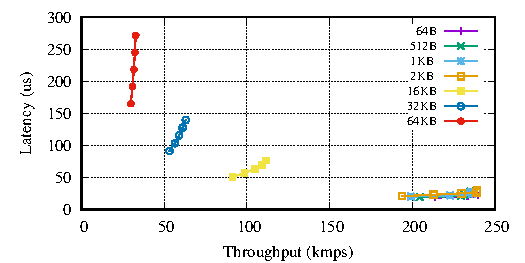
\includegraphics[width=0.99\columnwidth]{figures/benchmark/graphs/figure-performance-vs-size-single-group}
  \label{fig:tpcc_repartitioning}
  \end{subfigure}
  \begin{subfigure}{\columnwidth}
    \centering
    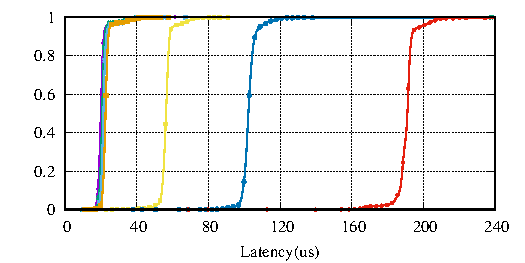
\includegraphics[width=0.95\columnwidth]{figures/benchmark/graphs/figure-performance-vs-size-single-group-cdf}
  \end{subfigure}
  \caption{Performance achieved with \libname with different message size; throughput versus latency (top) and the cumulative distribution function of latency measured when the system is saturated (bottom)}
\end{figure}

\subsection{Broadcast results}
\label{sec:evaluation:broadcast}

\begin{figure}[htp!]
  \begin{subfigure}{\columnwidth}
    \centering
    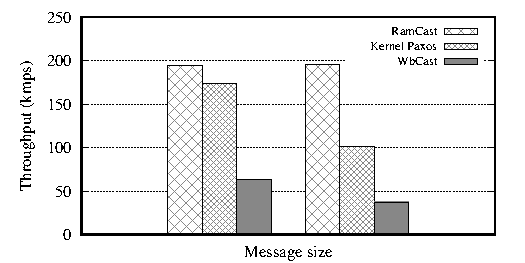
\includegraphics[width=0.99\columnwidth]{figures/benchmark/graphs/figure-compare-single-group-throughput}
  \label{fig:tpcc_repartitioning}
  \end{subfigure}
  \begin{subfigure}{\columnwidth}
    \centering
    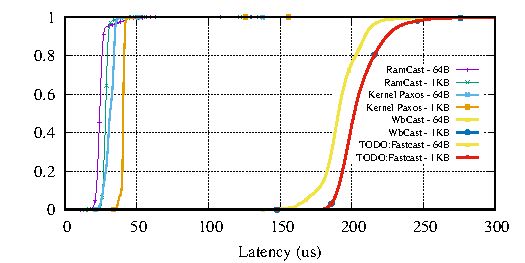
\includegraphics[width=0.95\columnwidth]{figures/benchmark/graphs/figure-compare-single-group-latency-cdf}
  \end{subfigure}
  \caption{Broadcasting performance comparison of \libname versus other protocols; throughput (top) and the cumulative distribution function of latency of a single client (bottom)}
\end{figure}

\begin{figure}[htp!]
  \begin{subfigure}{\columnwidth}
    \centering
    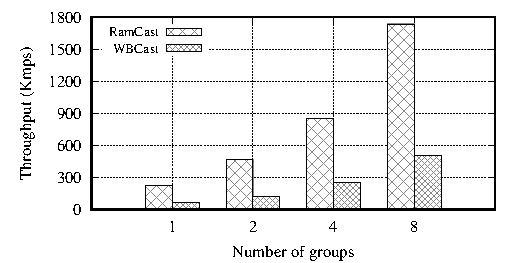
\includegraphics[width=0.99\columnwidth]{figures/benchmark/graphs/figure-genuine-compare-throughput}
  \label{fig:tpcc_repartitioning}
  \end{subfigure}
  \begin{subfigure}{\columnwidth}
    \centering
    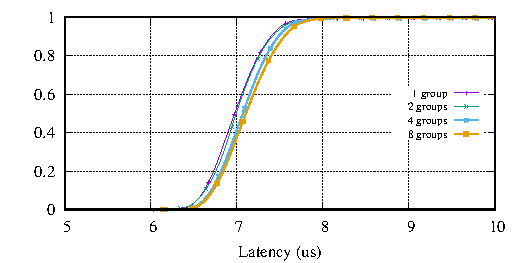
\includegraphics[width=0.95\columnwidth]{figures/benchmark/graphs/figure-genuine-compare-latency-cdf}
  \end{subfigure}
  \caption{Performance comparison of \libname versus other protocol for single group message; throughput (top) and the cumulative distribution function of latency of a \libname\'s single client (bottom)}
\end{figure}


\subsection{Multicast results: performance vs. number of destinations}
\label{sec:evaluation:multicast}


\begin{figure}[htp!]
  \begin{subfigure}{\columnwidth}
    \centering
    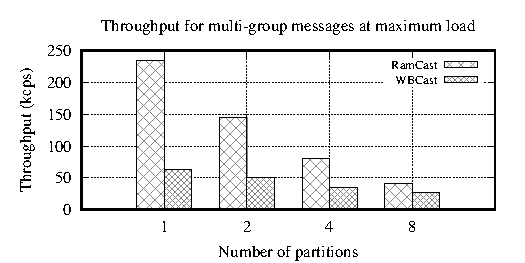
\includegraphics[width=0.99\columnwidth]{figures/benchmark/graphs/figure-multi-dest-compare-throughput}
  \label{fig:tpcc_repartitioning}
  \end{subfigure}
  \begin{subfigure}{\columnwidth}
    \centering
    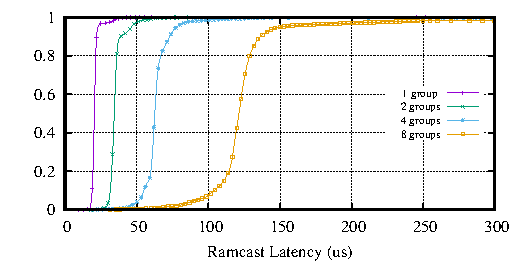
\includegraphics[width=0.95\columnwidth]{figures/benchmark/graphs/figure-multi-dest-compare-latency-cdf-ramcast}
  \end{subfigure}
  \begin{subfigure}{\columnwidth}
    \centering
    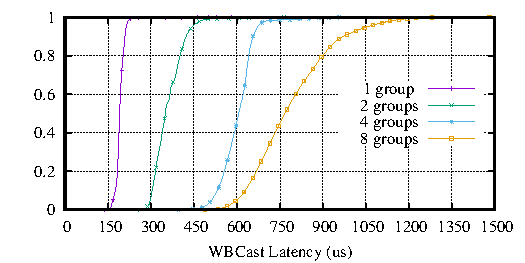
\includegraphics[width=0.95\columnwidth]{figures/benchmark/graphs/figure-multi-dest-compare-latency-cdf-wbcast}
  \end{subfigure}
  \caption{Performance comparison of \libname versus other protocol for multi groups message; throughput (top) and the cumulative distribution function of latency of a \libname\'s (middle) and WBCast (bottom)}
\end{figure}
